\documentclass[conference]{IEEEtran}
\IEEEoverridecommandlockouts
% The preceding line is only needed to identify funding in the first footnote. If that is unneeded, please comment it out.
\usepackage{cite}
\usepackage{amsmath,amssymb,amsfonts}
\usepackage[english]{babel}
\usepackage{algorithmic}
\usepackage{graphicx}
\usepackage{textcomp}
\usepackage{xcolor}
\usepackage{hyperref}
%\usepackage{algorithm}
\usepackage{algorithm2e}
\usepackage{algorithmic}
\DeclareMathOperator*{\argmin}{arg\,min}
\def\BibTeX{{\rm B\kern-.05em{\sc i\kern-.025em b}\kern-.08em
		T\kern-.1667em\lower.7ex\hbox{E}\kern-.125emX}}
\begin{document}
	
	\title{Efficient Hessian-Free Optimization of Deep Neural Networks
		%\\
		%{\footnotesize \textsuperscript{*}Note: Sub-titles are not captured in Xplore and
		%should not be used}
		%\thanks{Identify applicable funding agency here. If none, delete this.}
	}
	
	\author{\IEEEauthorblockN{Niklas Brunn}
		\IEEEauthorblockA{\textit{Albert Ludwigs University of Freiburg} \\
			\textit{Mathematical Institute}\\
			Freiburg, Germany \\
			niklasbrunn@web.de}
		\and
		\IEEEauthorblockN{No\"{e}l E. Kury}
		\IEEEauthorblockA{\textit{Albert Ludwigs University of Freiburg} \\
			\textit{Mathematical Institute}\\
			Freiburg, Germany \\
			nekury@wkury.de}
		\and
		\IEEEauthorblockN{Clemens A. Schächter}
		\IEEEauthorblockA{\textit{Albert Ludwigs University of Freiburg} \\
			\textit{Mathematical Institute}\\
			Freiburg, Germany \\
			clemens.schaechter@live.com}
	}
	
	\maketitle
	\thispagestyle{plain}
	\pagestyle{plain}
	
	\begin{abstract}
		This report is a written elaboration of a project which was developed in the lecture Numerical Optimization in the winter term 21/22 at the Albert-Ludwigs-University of Freiburg.\\
		We discuss a $2^{\text{nd}}$-order optimization method for training deep neural networks using the generalised Gauss-Newton Matrix as an approximation for the Hessian of the objective loss function. In addition, we present an implementation of the method using Python 3, Tensorflow and compare the results to a $1^{\text{st}}$-order optimization method (SGD) on the MNIST dataset.
	\end{abstract}
	
	\section{Introduction} 
		\noindent
	Deep neural networks (DNNs) are an important deep learning architecture and have a wide field of applications. When training a DNN, the network parameters are updated according to certain rules, which we call the DNN optimization method. Here stochastic gradient descent (SGD) is often used as such an optimization method. SGD is a $1^{\text{st}}$-order optimization method in which only the negative gradient of the object loss function (OL) with respect to the network parameters is used to update the current parameters.
	One problem of SGD is that pathological curvature of the OL is not considered. This means that the method can get stuck in saddle points, or often converges very slowly in environments with pathological curvature. \\ On the other hand
	$2^{\text{nd}}$-order optimization methods take into account the curvature of the OL and can thus circumvent such problems. But they are often costly in time because second order derivatives must be computed for this purpose. \\
	We want to use a version of Newton's method for DNN optimization as presented in [4].
	We use an approximation of the Hessian matrix, which is positive definite, and thus allows the use of the conjugate gradient (CG) method for determining parameter updates. Therefore we discuss the individual problems of standard Newton updates and the improvements proposed for them in order to ensure computational efficiency.\\
	Our own implementation of the method in Python 3 [9] with Tensorflow [1] can be accessed on GitHub \href{https://github.com/NiklasBrunn/Hessian_Free_Optimization_of_Deep_Neural_Networks}{(Github repository)}. Finally, we train a DNN on the MNIST-Dataset with SGD and the introduced $2^{\text{nd}}$-order optimization method and compare our results.
	
	
	\section{Optimization of Deep Neural Networks}
		\noindent
	In this section, we introduce the necessary mathematical notations for optimizing DNNs, formulate the parameter optimization task as a nonlinear programming problem (NLP) and explain tricks for the OL, which will be useful in the implementation of the presented optimization method.
	
	\subsection{Deep Neural Networks}
		\noindent
	A deep neural network is an an artificial neural network in wich additional layers between input and output layer provide some depth. They are often used as function approximators.\\ Given a dataset of observation pairs $D =\{(x_{i}, y_{i})_{1\leq i\leq N}\}$ with inputs ${x_i}$ and corresponding targets $y_i$, we aim to find a set of parameters so that the DNN's evaluations are approximately the corresponding observed targets $y_i$.\\ \ \\  Given a fixed input $x$, the realization
	of a DNN is a mapping
	\begin{align}
	&R_{x}:\Theta^{d}\rightarrow\mathbb{R}^{m}\\
	&\theta\mapsto R_{x}(\theta)=:z_{x}
	\end{align}
	Here $\theta$ is a vector containing the parameters of our network with parameter space $\Theta^{d}=\mathbb{R}^{d}$ and output $z_{x} =R_{x}(\theta)$.\\ The realization is an alternating concatenation of a fixed number of affine and nonlinear mappings with respect to its input $x$. The parameter vector $\theta$ is the collection of every entry of all weight matrices and bias vectors in the affine mappings.\\ These affine mappings are called layers and the nonlinear mappings are called activation functions. Activation functions $\varrho:\mathbb{R}\rightarrow\mathbb{R}$ are one dimensional, nonlinear, real valued functions which are applied element-wise to the activation of the preceding layer. Usually the same activation function is applied to all hidden layers of the network. \\
	We assume that an additional activation function $\phi:\mathbb{R}\rightarrow\mathbb{R}$ can be applied to the DNNs output which is not considered as a component of the network architecture. This allows us to use technical tricks that later favor our implementation.
	We denote
	\begin{align}
	\hat{y}_{x} := \phi(z_{x}).
	\end{align}
	which serves as approximation to $y$.\\
	We also allow $\phi$ to be the identity function for cases in which no further mapping of the network output is needed.
	
	\subsection{Loss functions}
	\noindent
	For parameter optimization it is important to choose a scalar-valued loss function
	\begin{align}
	&L:\mathbb{R}^{m}\times \mathbb{R}^{n}\rightarrow \mathbb{R}^{+};\\
	&(x, y)\mapsto L(x, y).
	\end{align}
	Further we define the output loss function
	\begin{align}
	&L_{y}:\mathbb{R}^{m}\rightarrow \mathbb{R}^{+};\\
	&z\mapsto L_{y}(z) := L(z, y),
	\end{align}
	which is asumed to be at least twice continuous-differentiable in $z$. The output loss takes $z_{x}$ as input for a fixed target $y$ which corresponds to the observed value $x$ and can be seen as a feedback signal, how well the DNN fits the observation data with its current parameters. Choosing a good loss function is an important tasks in the optimization of DNNs. In our multi-classification task we use the cross-entropy loss function with softmax-activation on the output layer. 
	\textbf{Definieren!}
	
	\subsection{Network training formulated as a NLP}
	Parameter optimization of a DNN can be formulated as an unconstrained NLP. Therefore we define the OL as a mapping which calculates the empirical loss of the DNN`s output with current parameters $\theta$ given the input $x$ and the corresponding target $y$
	\begin{align}
	&f_{D}:\Theta^{d}\rightarrow\mathbb{R}^{+},\\
	\theta\mapsto f_{D}(\theta) &:= \mathbb{E}_{D}[L_{y}(z_{x})] =  \frac{1}{N}\sum_{j = 1}^{N}L_{y_{j}}(z_{x_{j}}).
	\end{align}
	Thus we get the unconstrained NLP formulation
	\begin{align}
	\argmin_{\theta\in\Theta^{d}}\quad f_{D}(\theta),
	\end{align}
	where $\theta$ denotes the decision variable and $f_{D}$ the objective function of the NLP.
	Further, if we consider a single observation $(x, y)$ from the observation data set $D$, we write  $f_{x, y}$ for the corresponding OL. Note that the above formulated NLP is typically non-convex due to the non-convexity of the OL.
	
	\subsection{Matching loss functions}
	For later purposes we need to calculate the Jacobian or the gradient of the OL with respect to the DNNs parameters. For simplicity we consider the OL for only one pair of observations
	\begin{align}
	J_{f_{x, y}} := \frac{\partial}{\partial\theta}f_{x, y}(\theta).
	\end{align}
	and neglect the dependency to the parameters $\theta$ to ensure readability.
	The results can be extended without problems to a case where the whole data set or a batched version of the whole data set is considered due to linearity of the derivative.
	Applying the chain rule we can rewrite the Jacobian in (11) to
	\begin{align}
	J_{f_{x, y}} &= J_{L_{y}\circ \:\phi \:\circ\:R_{x}} = J_{L_{y}} \: J_{\phi} \: J_{R_{x}},\\
	J_{f_{x, y}}^{\mathrm{T}} &= J_{R_{x}}^{\mathrm{T}} \: J_{\phi}^{\mathrm{T}} \: J_{L_{y}}^{\mathrm{T}}.
	\end{align}
	As introduced in [8], we also make use of so-called matching loss functions. We say that a loss function $L$ matches the output-non-linearity $\phi$ if
	\begin{align}
	\frac{\partial}{\partial\hat{y}_{x}}\left(L_{y}\circ \phi\right)^{\mathrm{T}}(\hat{y}_{x})= J_{L_{y}\circ \:\phi}^{\mathrm{T}} = A\: z_{x} + b,
	\end{align}
	for a matrix $A$ and vector $b$, which both do not depend on the parameters $\theta$.
	Cross-entropy loss with softmax-activation matches their nonlinear output. 
	%We will see that many of the well known loss functions used for DNN optimization match %their output-nonlinearity, e.g. the squared error loss function and crossentropy loss %function with previous softmax-activation function.
	
	
	\section{Hessian-Free optimization method}
	In this section we want to give the reader a brief introduction to the Stochastic Generalized Gauss-Newton Method. For a more detailed discussion in Newton-type optimization we refer the reader to chapter 7 in [2]. For details about problems with pathological curvature to [4]. And for information about the Generalised Gauss Newton matrix to chapter 8 in [5].
	
	\subsection{Newton's method}\label{AA}
	Newton`s method is an optimization method, where we update the decision variables of our NLP formulation in (10) iteratively by
	\begin{align}
	\theta_{k+1} = \theta_{k} -H_{f_{x, y}}(\theta_{k})^{-1}\cdot J_{f_{x, y}}^{\mathrm{T}}(\theta_{k}).
	\end{align}
	Here $H_{f_{x, y}}(\theta_{k})$ denotes the Hessian of the OL with respect to the current DNNs parameters $\theta_{k}$. One can obtain this by minimizing the local quadratic approximation
	\begin{align}
	q_{\theta_{k}}(\delta)&:= f_{x, y}(\theta) + J_{f_{x, y}}^{\mathrm{T}}\:\delta + \frac{1}{2}\:\delta^{\mathrm{T}}\:H_{f_{x, y}}(\theta)\:\delta\\
	&\approx f_{x, y}(\theta + \delta)
	\end{align}
	with respect to $\delta$. 
	Using Newton's method can lead to convergence in fewer iterations compared with gradient descent. This is because it rescales the gradient of the OL in every step by using information about the local curvature of the OL. This makes Newton's method less susceptible to pathological curvature, where first order gradient-based methods like SGD can get stuck in saddle points. We will also hide the dependency on the parameters $\theta$ in our notation of the Hessian and Hessian approximations.
	
	\subsection{Problems with the Hessian}
	We implicitly assume in every step (15) that the Hessian is invertible, which sometimes is not the case in our task (10). Also, we can not ensure converges to a local minimum, since the Hessian can not assumed to be positive semi definite either. Furthermore the Hessian has $d^{2}$ entries consisting of second-order partial derivatives, which makes it very expensive to calculate, whenever $d>>m$. For these reasons the direct application of Newton's method to our task is not feasible. We therefore discuss some modifications to ensure an efficient application of Newton`s method.
	
	\subsection{The Generalized Gauss Newton Matrix}
	We no longer use the Hessian itself, but the Generalized Gauss Newton matrix (GGN), which is an approximation of the Hessian 
	\begin{align}
	G_{f_{x, y}} := J_{R_{x}}^{\mathrm{T}}\:H_{L_{y}\circ\:\phi}\:J_{R_{x}},
	\end{align}
	where $H_{L_{y}\circ\:\phi}$ denoties the Hessian of $L_{y}\circ\:\phi$ with respect to $\hat{y}_{x}$ and $J_{R_{x}}$ denoting the Jacobian of the realisation of the DNN with respect to its parameters.
	Regarding the full Hessian of the OL
	%This representation is motivated by the fact that in the representation of the complete %Hessian of the OL
	\begin{align}
	H_{f_{x, y}} = J_{\hat{y}_{x}}^{\mathrm{T}}\:H_{L_{y}\circ\:\phi}\:J_{\hat{y}_{x}}\:\sum_{j = 1}^{m}\left(\left(J_{L_{y}\circ \:\phi}^{\mathrm{T}}\right)_{j}\cdot H_{(\hat{y}_{x})_{j}}\right),
	\end{align}
	where $H_{(\hat{y}_{x})_{j}}$ denotes the Hessian of the DNN`s  $j$-th output, the last sum-term vanishes if one of the two factors in the sum of (19) vanishes.
	%\begin{align}
	%\left(J_{L_{y}\circ \:\phi}^{\mathrm{T}}\right)_{j}\approx 0\:\lor\:H_{(\hat{y}_{x})_{j}} \approx 0.
	%\end{align}
	This means that for a local optimum $\theta^{\star}$ we have $H_{f_x, y} \approx G_{f_x, y}$.   Moreover, the GGN is a symmetric and positive semi definite matrix by construction if $L_{y}\circ\:\phi$ is convex, since for every $v\in\mathbb{R}^{d}$ it holds that
	\begin{align}
	v^{\mathrm{T}}\:G_{f_{x, y}}\:v &= v^{\mathrm{T}}\:\left( J_{\hat{y}_{x}}^{\mathrm{T}}\:H_{L_{y}\circ\:\phi}\:J_{\hat{y}_{x}}\right)\:v\\
	&= \left(J_{\hat{y}_{x}}\:v\right)^{\mathrm{T}}H_{L_{y}\circ\:\phi}\left(J_{\hat{y}_{x}}\:v\right) \\
	&\geq 0.
	\end{align}
	For cross-entropy loss with softmax-activation it holds that $L_{y}\circ\:\phi$ is convex.
	
	\subsection{Levenberg-Marquardt algorithm }
	To ensure invertibility %Thus it it sometimes not possible to find a solution of the linear system
	%\begin{align}
	%G_{f_{x, y}}\cdot(\theta_{k+1} - \theta_{k}) = -J_{f_{x, y}}^{\mathrm{T}},
	%\end{align}
	%which is equivalent to the system stated in (15) using the GGN insted of the Hessian.
	we use a damped version of the GGN (DGGN). Using Levenberg-Marquardt technique, where we add an diagonal matrix with positive values on the diagonal, e. g.
	\begin{align}
	DG_{f_{x, y}} := G_{f_{x, y}} + \lambda\cdot I^{d\times d},
	\end{align}
	with $I^{d\times d}$ denoting the $d\times d$ unit matrix and some $\lambda>0$.
	The DGGN constructed this way is always positive definite. 
	We consider the decomposition
	\begin{align}
	G_{f_{x, y}} = U\:\Lambda\:U^{\mathrm{T}},
	\end{align}
	with an orthogonal Matrix $U\in\mathbb{R}^{d\times d}$ and a diagonal Matrix $\Lambda\in\mathbb{R}^{d\times d}$ which on the diagonal entries contains the nonnegative eigenvalues of the GGN. This decomposition exists because the GGN is symmetric and positive semidefinite. Further it holds that
	\begin{align}
	DG_{f_{x, y}} &= U\:\Lambda\:U^{\mathrm{T}} + \lambda\cdot I^{d\times d}\\
	&= U\:\Lambda\:U^{\mathrm{T}} + U\:\lambda\cdot I^{d\times d}\:U^{\mathrm{T}}\\
	&= U\:\left(\Lambda + \lambda\cdot I^{d\times d}\right)\:U^{\mathrm{T}}
	\end{align}
	where the matrix $\left(\Lambda + \lambda\cdot I^{d\times d}\right)$ is a diagonal one with only positive entries on its diagonal. Therefore the determinant of (27) is positive which implies that the DGGN is positive definite and invertible.
	Note that a choice of $\lambda>>0$ leads to a Newton step where the change of our parameters is marginal. On the other hand $\lambda\approx 0$ leads to a full step using the GGN. In practice, we update the value $\lambda$ after each iteration and should thus be denoted by $\lambda_{k}$. Following [4] we define the reduction ration
	\begin{align}
	\rho := \frac{f_{B}(\theta_{k}) - f_{B}(\theta_{k+1})}{q_{\theta_{k}}(\Delta\theta_{k + 1}) - q_{\theta_{k}}(0)}
	\end{align}
	and then update the value $\lambda_{k}$ according to the rule
	\begin{align}
	&\textbf{if}\:\rho<\frac{1}{4}:\\
	&\text{ }\text{ }\text{ }\text{ }\lambda_{k+1} = r\cdot\lambda_{k}\\
	&\textbf{elif}\:\rho>\frac{3}{4}:\\
	&\text{ }\text{ }\text{ }\text{ }\lambda_{k + 1} = r^{-1}\cdot\lambda_{k}\\
	&\textbf{else}: \\
	&\text{ }\text{ }\text{ }\text{ }\lambda_{k + 1} = \lambda_{k}\\
	&\textbf{return}:\:\lambda_{k + 1},
	\end{align}
	where $r=1.5$.
	In our experiments we found that for a smaller batch size $(N<150)$ it is critical to adjust the update amount of the damping value to a smaller size, e. g. $r=1.01$, to ensure stable convergence.
	For large batch sizes $r=1.01$ leads to slower convergence.
	
	\begin{figure}[htbp]
		\centerline{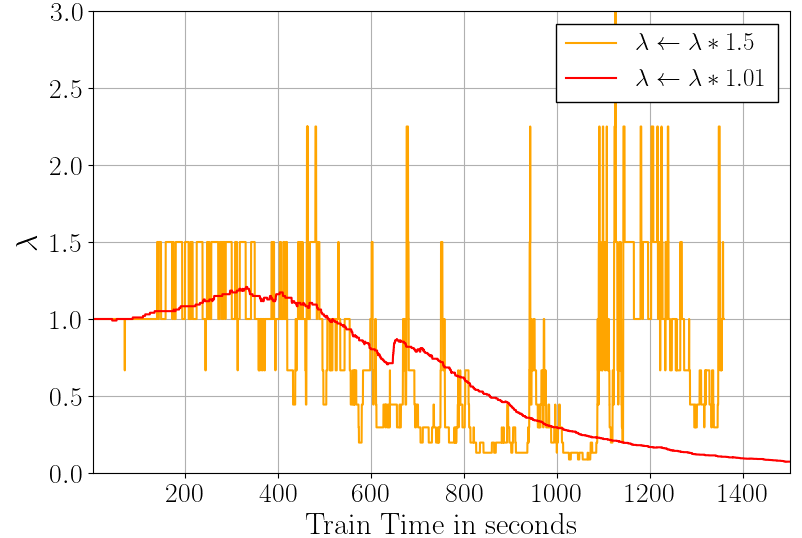
\includegraphics[scale=0.52]{lambda.png}}
		\caption{$\lambda$ during training with batch size $75$ and $r=1.5$ (orange) and $r=1.01$ (red). A large $r$ is unstable due to the stochasticity of the mini batch sampling. This leads to unstable convergence.}
		\label{fig}
	\end{figure}
	
	\subsection{Conjugate Gradient method}
	Computing the parameter updates in (15) directly using the DGGN would be very inefficient becaus we need to calculate and store the invers of the DGGN. Instead we reformulate the equation in (15) to an equivalent formulation
	\begin{align}
	DG_{f_{x, y}}(\theta_{k})\cdot\Delta\theta_{k+1} &= -J_{f_{x, y}}^{\mathrm{T}}(\theta_{k}),\\
	%DG_{k}^{f_{x, y}}\:\Delta\theta_{k+1} &= -(J_{k}^{f_{x, y}})^{\mathrm{T}},\\
	\Delta\theta_{k+1} :&= \theta_{k+1} - \theta_{k}
	\end{align}
	and approximate the solution to this linear equation system using a preconditioned version of the Conjugate gradient (CG) method, where we use the results that are discussed in [4]. 
	This approach allows us to efficiently approximate the parameter updates with at most $d$ steps, without calculating and storing the DGGN once at any time. Instead we use efficient matrix-vector products to calculate the product of the DGGN with an vector whenever necessary. Since in our task $d>>0$, we do not iterate until convergence but instead terminate the iterations after a minimum number of steps, if certain termination criteria are met. It is worth mentioning that in our experiments a minimum number of 3 CG-steps works well even if we have $d=397.510$ or larger. 
	
	\subsection{Mini-batches}
	If we are facing a large observation data set with $N>>0$, it is common to split the data set into batches $B\subset D$ containing only a few random samples $M<<N$ of the entire data and apply the optimization algorithm to each of the generated batches for each iteration. The partition of $D$ into smaler batches is called a mini-batch szenario, where $M$ denotes the batchsize of the mini-batches. For each mini-batch $B$ the DGGN in (23) becomes
	\begin{align}
	DG_{f_{B}} := \frac{1}{M}\sum_{(x, y)\in B}^{}G_{f_{x, y}} + \lambda\cdot I^{d\times d}.
	\end{align}
	As mentioned in [3], the batch size should be relatively large to capture enough information about the curvature of the OL and for to ensure stability in optimization . 
	
	
	
	\section {Implementation}
	For the implementation of the Hessian-Free optimization method, we will first explain in more detail the previously mentioned tricks for an efficient computation of matrix-vector-products and specifically discuss the use of pre-implemented commands for FAD and BAD in Tensorflow. Only the recently added Tensorflow command for FAD makes it possible to implement the method efficiently in Tensorflow.
	
	
	\subsection{Efficient computation of matrix-vector-products}
	For the implementation of the Hessian-Free optimization method we use an efficient way to calculate matrix-vector-products in the CG-iterations. Note that the only time where we need to compute a matrix-vector-product is in each CG-iteration once and additionally one time for the full CG-run. This idea was first presented in [8] using results from [7]. We now consider the product of the DGGN with an arbitrary vector $v$ that we want to compute in an efficient way.
	Therefore we make use of FAD and BAD since it is well known (e.g. chapter 10 in [2]) that for a vector valued function $F:\mathbb{R}^{n}\rightarrow\mathbb{R}^{m}$ we can compute the Jacobian-vector-product at a cost of only
	\begin{align}
	\mathrm{cost}_{\text{FAD}}(J_{F}\:v)\leq 2\:\mathrm{cost}(F),\\
	\mathrm{cost}_{\text{BAD}}(J_{F}^{\mathrm{T}}\:v)\leq 3\:\mathrm{cost}(F).
	\end{align}
	For matching loss functions we get from (14)
	\begin{align}
	H_{L_{y}\circ\:\phi} &= \frac{\partial}{\partial \hat{y}_{x}}J_{L_{y}\circ\:\phi}^{\mathrm{T}} \\
	%= \frac{\partial}{\partial \hat{y}_{x}}(A\:z_{x} + b)\\ 
	&= A\:J_{\phi} \\
	&= J_{\phi}^{\mathrm{T}}\:A^{\mathrm{T}}.
	\end{align}
	This identity makes it much easier for us to compute the DGGN, since in this case we do not need to compute the Hessian. In summary, we want to calculate the following matrix-vector product
	\begin{align}
	DG_{f_{B}}\:v &=  \left(J_{\hat{y}_{x}}^{\mathrm{T}}\:A\:J_{\phi}\:J_{\hat{y}_{x}} + \lambda\cdot I^{d\times d}\right)\:v\\
	&= J_{\hat{y}_{x}}^{\mathrm{T}}\:A\:J_{\phi\circ R _{x}}\:v + \lambda\cdot I^{d\times d}\:v
	\end{align}
	Here we can compute the first part of the sum in (37) using Tensorflow's pre-implemented functions for FAD and BAD. By this we mean that we first compute the outputs of the DNN given the current parameters and afterwards evaluate the Jacobi-vector-product 
	\begin{align}
	u := J_{\phi\circ R _{x}}\:v,
	\end{align}
	followed by an left multiplication with the matrix $A$ and then compute the product 
	\begin{align}
	J_{R_{x}}^{\mathrm{T}}\:w
	\end{align}
	using BAD, where $w := A\:u$. Also note that using (35) insted of (34) we get 
	\begin{align}
	DG_{f_{B}}\:v  = J_{\phi\circ R _{x}}^{\mathrm{T}}\:A\:J_{R _{x}}\:v + \lambda\cdot I^{d\times d}\:v.
	\end{align}
	In contrast to (37), here we put more of the differentiation task in the backward pass. 
	%In general if we dont have a matching loss function we get 
	%\begin{align}
	%DG_{f_{B}}\:v &= \left(J_{R_{x}}^{\mathrm{T}}\:H_{L_{y}\circ\:\phi}\:J_{R_{x}} + \lambda\cdot %I^{d\times d}\right)\:v\\
	%& = J_{R_{x}}^{\mathrm{T}}\:H_{L_{y}\circ\:\phi}\:J_{R_{x}}\:v + \lambda\cdot I^{d\times d}\:v
	%\end{align}
	%and compute the left term of the sum in (42) by again first evaluating the DNN`s output given $x$ with the current parameters and after that evaluate the Jacobi-vector-product 
	%\begin{align}
	%u := J_{R _{x}}\:v,
	%\end{align}
	%then using FAD after BAD to compute the product 
	%\begin{align}
	%w := H_{L_{y}\circ\:\phi}\:u 
	%\end{align}
	%and finally compute 
	%\begin{align}
	%J_{R_{x}}^{\mathrm{T}}\:w
	%\end{align}
	%using BAD. 

	
	\subsection{Tensorflow}
	We implement our version of the Hessian-Free method in Tensorflow [1] because it is one of the widly used packages for Machine Learning.
	We make use of Tensorflows pre-implemented FAD-command \href{https://www.tensorflow.org/api_docs/python/tf/autodiff/ForwardAccumulator}{tf.autodiff.ForwardAccumulator} and BAD-command \href{https://www.tensorflow.org/api_docs/python/tf/GradientTape}{tf.GradientTape}. Our code is avilable at our github repository \href{https://github.com/NiklasBrunn/Hessian_Free_Optimization_of_Deep_Neural_Networks}{(Github repository)}.
	
	
	

	TODO: ALGORITHMS (FAST-MAT-VEC-Pseudocode und CG-Pseudocode)
	
	\RestyleAlgo{ruled}
	
	\begin{algorithm}
	\SetKwInOut{Input}{Input}
	\SetKwInOut{Output}{Output}
	\SetKwInOut{CG}{\textbf{pre-CG-result}}
	\SetKwInOut{LAM}{\textbf{$\lambda$-update($B$, $\Delta\theta_{k+1}$, $\lambda$)}}
	\caption{Fast DGGN-Vector Product}\label{alg:one}
	\Input{Network Parameters $\theta_k$, Mini-Batch $B$, Vector $v$}
	...
	\Output{$(G+I\lambda_k)v$}
	\end{algorithm}	

	
	\begin{algorithm}
		\SetKwInOut{Input}{Input}
		\SetKwInOut{Output}{Output}
		\SetKwInOut{CG}{\textbf{pre-CG-result}}
		\SetKwInOut{LAM}{\textbf{$\lambda$-update($B$, $\Delta\theta_{k+1}$, $\lambda$)}}
		\caption{Hessian-Free pseudocode for (10)}\label{alg:one}
		\Input{$D$, $\theta_{0}$, $\lambda$, epochs}
		\For{epoch in epochs}{
			$k\gets 0$\\
			\For{$(x, y)$ in $D$}{
				$J_{f_{x, y}}^{\mathrm{T}}(\theta_{k})\:$(compute with BAD)\\
				\CG{$\Delta\theta_{k+1}$}
				$\theta_{k+1}\gets \theta_{k} + \Delta\theta_{k+1}$\\
				\LAM{$\lambda$}
				$k\gets k+1$
			}	
			$\theta_{0} \gets \theta_{N}$
		}
		\Output{$\theta^{trained}$}
	\end{algorithm}
	
	\begin{algorithm}
		\SetKwInOut{Input}{Input}
		\SetKwInOut{Output}{Output}
		\SetKwInOut{CG}{\textbf{pre-CG-result}}
		\SetKwInOut{LAM}{\textbf{$\lambda$-update($B$, $\Delta\theta_{k+1}$, $\lambda$)}}
		\caption{(Mini-batch)-Hessian-Free pseudocode for (10)}\label{alg:two}
		\Input{$D_{\mathrm{batched}}$, $B$, $\theta_{0}$, $\lambda$, epochs}
		\For{$epoch$ in epochs}{
			$k\gets 0$\\
			\For{$B$ in $D_{\mathrm{batched}}$}{
				$J_{f_{B}}^{\mathrm{T}}(\theta_{k})\:$(compute with BAD)\\
				\CG{$\Delta\theta_{k+1}$}
				$\theta_{k+1}\gets \theta_{k} + \Delta\theta_{k+1}$\\
				\LAM{$\lambda$}    
				$k\gets k+1$
			}
			$\theta_{0}\gets \theta_{\frac{N}{M}}$	
		}
		\Output{$\theta^{trained}$}
	\end{algorithm}
	
	\begin{algorithm}
		\SetKwInOut{Input}{Input}
		\SetKwInOut{Output}{Output}
		\SetKwInOut{CG}{\textbf{pre-CG-result}}
		\SetKwInOut{LAM}{\textbf{$\lambda$-update}}
		\SetKwInOut{FMV}{\textbf{fast-mat-vec-out($B$, $\Delta\theta_{k+1}$, $\lambda$)}}
		\caption{Condition for $\lambda$-updates}\label{alg:three}
		\Input{$\Delta\theta_{k+1}$, $f_{B}(\theta_{k})$ $DG_{f_{B}}(\theta_{k})\:\Delta\theta_{k+1}$}
		$loss_{\mathrm{old}}\gets f_{B}(\theta_{k})$\\
		$loss_{\mathrm{new}}\gets f_{B}(\theta_{k}+\Delta\theta_{k+1})$\\
		$A\:\Delta\theta_{k+1}\gets DG_{f_{B}}(\theta_{k})\:\Delta\theta_{k+1}$\\
		$denom \gets J_{f_{B}}^{\mathrm{T}}\cdot\Delta\theta_{k+1} + \frac{1}{2}\Delta\theta_{k+1}^{\mathrm{T}}A\:\Delta\theta_{k+1}$
		$\rho\gets loss_{\mathrm{old}}\:-\:loss_{\mathrm{new}}\cdot(denom)^{-1}$\\
		\text{}\\
		\If{$\rho<\frac{1}{4}$}{$\lambda\gets \frac{3}{2}\:\lambda$}
		\ElseIf{$\rho>\frac{3}{4}$}{$\lambda\gets \frac{2}{3}\:\lambda$}
		\Output{$\lambda$}
	\end{algorithm}
	
	\begin{algorithm}
		\SetKwInOut{Input}{Input}
		\SetKwInOut{Output}{Output}
		\SetKwInOut{CG}{\textbf{pre-CG-result}}
		\SetKwInOut{LAM}{\textbf{$\lambda$-update($B$, $\Delta\theta_{k+1}$, $\lambda$)}}
		\caption{Fast matrix-vector produkts (DGGN multiplied with an arbitrary vector $v$)}\label{alg:four}
		\Input{$B$, $v$, $\lambda$, $\theta_{k}$}
		$G_{f_{B}}(\theta_{k})\:v$ (compute with FAD and BAD)\\
		$DG_{f_{B}}(\theta_{k})\: v \gets G_{f_{B}}\: v + \lambda\cdot I^{d\times d}\:v$\\
		\Output{$DG_{f_{B}}(\theta_{k})\: v$}
	\end{algorithm}
	
	\begin{algorithm}
		\SetKwInOut{Input}{Input}
		\SetKwInOut{Output}{Output}
		\SetKwInOut{CG}{\textbf{pre-CG-result}}
		\SetKwInOut{LAM}{\textbf{$\lambda$-update($B$, $\Delta\theta_{k+1}$, $\lambda$)}}
		\caption{(preconditioned) CG method}\label{alg:five}
		
	\end{algorithm}
	\section{Experiments}
	\noindent
	To test our implementation we use the MNIST-Dataset.
	It consists of grayscale images of handwritten digits from $0$ to $9$, with a resolution of $28\times28$ pixels. We flatten each image to a vector of size $784$ and divide by $255$, which transforms the data to $[0,1]^{784}$.\\ The train data set consists of $60,000$ images. For validation we use the test data set with $10,000$ images.\\ 
	For our DNN we chose an architecture with one hidden layer with $800$ Neurons. The total Number of trainable Parameters is $636,010$.\\
	\\ \ \\ We train the model on a Asus F571 Laptop with 16GB RAM, Intel Core i5-9300H and GeForce GTX 1650 4GB VRAM.
	
	\noindent
	For Stochastic Gradient Descent we chose as Learning Rate $\eta=0.1$ and Batch Size $N=100$. We also tested $\eta=0.01$, $\eta=0.025$ and $\eta=0.3$ as well as $N=250$. But it achieved worse results. \\
	The SGD benchmark for this model architecture with cross-entropy loss without data pre-processing, distortion, weight-decay etc. is an error rate of $1.6\%$ on the test data set. [10] 
	It can be achieved by initially setting the learning rate to $\eta=0.05$ and multiply it by $0.3$ every $100$ epochs. But convergence with these hyper-parameters is very slow.	
	\begin{figure}[htbp]
	\centerline{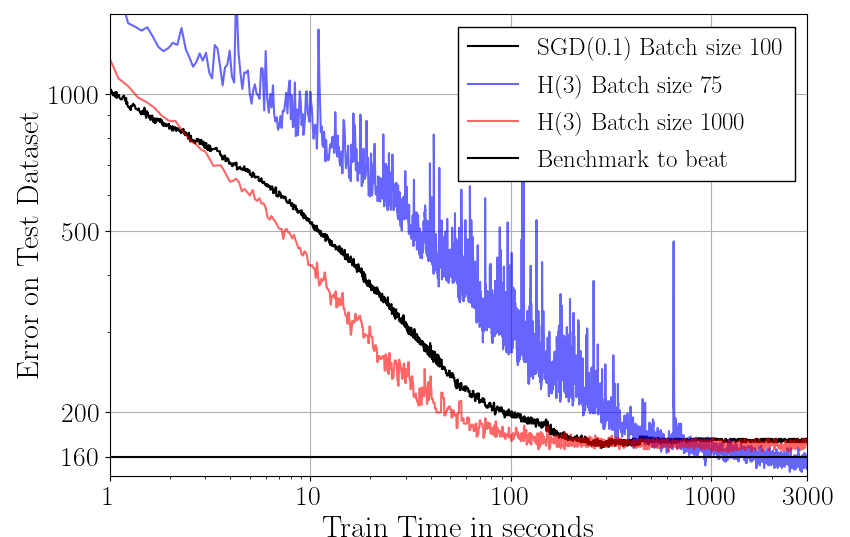
\includegraphics[scale=0.52]{Plot_Batch_size.png}}
	\caption{Comparison with SGD (black) and the effect of the batch size on performance. On the $y$-axis the total number of wrongly classified images on the whole test dataset is plotted. The corresponding train time to reach this result is plotted on the $x$-axis.}
	\label{fig}
	\end{figure}	

	We set $\varepsilon=0.0005$ and the number of minimal CG-steps to $3$. In practice the CG-method converges after $6-10$ steps. A higher minimal CG-step number e. g. $10$ does not lead to better performance, but need significantly more time for one total update step. Here CG-method converges after $13-17$ steps.\\
	With a large batch size $(N=1000)$ the method converges faster than SGD$(0.1), N=100.$ But SGD seems to converge more stable. After some time both methods tend to overfit on the train data. Here the total error converges to $0$, which effectively stops any improvement gains on the train dataset.\\
	With a small batch size $(N=75)$ the method converges much slower than SGD$(0.1)$ and seems to be very unstable. But the instability prevents overfitting to the train data. At around $1000$ seconds the method passes SGD and at $2000$ seconds the method consistently beats the Benchmark. After around $3000$ seconds the best performance measured is a $1.46\%$ error rate but due to the stochasticity of mini batching can get as high as $1.62\%$ on some batches. Because minor performance gains are still noticeable it may be possible to achieve an even better error rate. \\
	
	\begin{figure}[htbp]
	\centerline{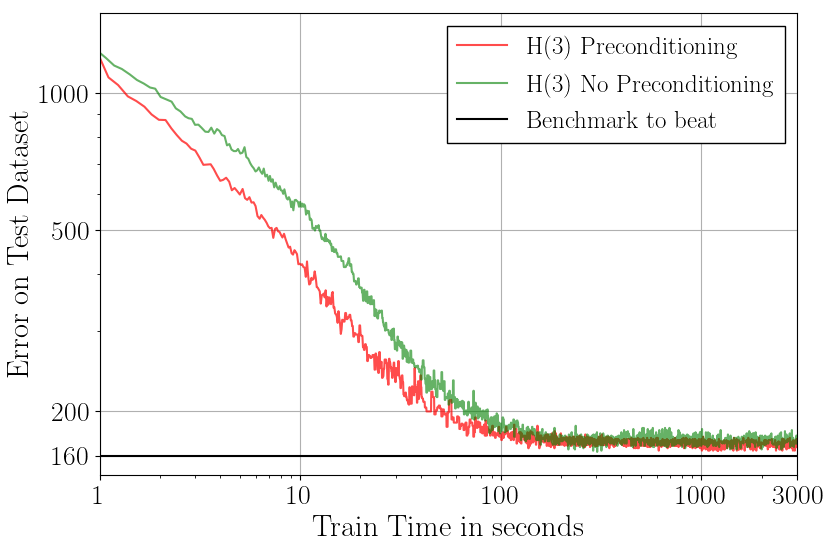
\includegraphics[scale=0.53]{Precond.png}}
	\caption{Effect of Preconditioning in the CG-method. Without Preconditioning convergence is slower. (Tested with $N=100$)}
	\label{fig}
	\end{figure}		
	\section*{Acknowledgment}
	I want to thank my cat. 
	

	
	
	\begin{thebibliography}{00}
		\bibitem{b1} M. Abadi, A. Agarwal, P. Barham, E. Brevdo,
		Z. Chen, C. Citro, G. S. Corrado, A. Davis,
		J. Dean, M. Devin, S. Ghemawat, I. Goodfellow,
		A. Harp, G. Irving, M. Isard, R. Jozefowicz, Y. Jia,
		L. Kaiser, M. Kudlur, J. Levenberg, D. Mané, M. Schuster,
		R. Monga, S. Moore, D. Murray, C. Olah, J. Shlens,
		B. Steiner, I. Sutskever, K. Talwar, P. Tucker,
		V. Vanhoucke, V. Vasudevan, F. Viégas,
		O. Vinyals, P. Warden, M. Wattenberg, M. Wicke,
		Y. Yu, and X. Zheng.
		TensorFlow: Large-scale machine learning on heterogeneous systems, Software available from tensorflow.org, 2015	
		\bibitem{b2} M. Diehl, "Lecture Notes on Numerical Optimization (Preliminary Draft)", Albert Ludwigs University of Freiburg, September 29, 2017	
		\bibitem{b3} M. Gargiani, A. Zanelli, M. Diehl, F. Hutter, "On the Promise of the Stochastic Generalized Gauss-Newton Method for Training DNNs",  arXiv:2006.02409v4, June 9, 2020 
		\bibitem{b4} J. Martens, "Deep learning via Hessian-free optimization", University of Toronto, Ontario, M5S 1A1, Canada, 2010
		\bibitem{b5} J. Martens, "New Insights and Perspectives on the Natural Gradient Method", Jurnal of Machine Learning Research 21, arXiv:1412.1193v11, September 19, 2020
		\bibitem{b6} J. Martens, I. Sutskever, "Training Deep and Recurrent Networks with Hessian-Free Optimization", In: G. Montavon, G.B. Orr, KR. Müller (eds), Neural Networks: Tricks of the Trade. Lecture Notes in Computer Science, vol 7700. Springer, Berlin, Heidelberg, 2012
		\bibitem{b7} B. A. Pearlmutta, "Fast Exact Multiplication by the Hessian", Neural Computation, June 9, 1993
		\bibitem{b8} N. N. Schraudolph, "Fast Curvature Matrix-Vector Products for Second-Order
		Gradient Descent", Neural Computation, August 2002
		\bibitem{b9} G. Van Rossum, F. L. Drake, Python 3 Reference Manual. Scotts Valley, CA: CreateSpace, 2009
		\bibitem{b10} https://en.wikipedia.org/wiki/MNIST\_database
	\end{thebibliography}
	
